\section{Introduction}

%智能家居是物联网的一个重要应用,随着物联网的发展走进更多用户的事业。智能家居包含自动化功能,允许用户去下载或者自定义自动化规则来让生活更加轻松舒适。
Smart home is an important application of the Internet of Things, and with the development of the Internet of Things, it has entered the field of more users. Smart homes include automation features that allow users to download or customize automation rules to make life easier and more comfortable.\cite{example}

%自动化规则通常由三个部分组成:触发器、条件判断、执行动作。例如在房间安装温度传感器、空调,设置自动化规则$\langle$ \text{ indoor temperature is below 24 degrees Celsius },\text{air conditioner is off },\text{trun on the air conditioner and set the air conditioner temperature to 27 degrees Celsius } $\rangle$ 表示当室内温度低于24摄氏度时,如果空调关闭,开启空调,,设定空调温度为27摄氏度从而实现室内恒温的功能。
Automation rules typically consist of three parts: triggers, conditional judgments, and execution actions. For example, installing a temperature sensor and air conditioner in a room, and setting the automation rule $\langle$ \texttt{ indoor temperature is below 24 degrees Celsius },\texttt{air conditioner is off },\texttt{trun on the air conditioner and set the air conditioner temperature to 27 degrees Celsius } $\rangle$ means that when the indoor temperature is below 24 degrees Celsius, if the air conditioner is off, turn on the air conditioner and set the air conditioner temperature to 27 degrees Celsius to achieve the function of constant indoor temperature.

%然而,多条自动化规则的执行可能会引发用户预期之外的操作,多条规则的交互可能会导致规则冲突从而带来严重的安全威胁。例如Fig.\ref{rule_conflict_example}中展示的两条规则。Automation 1 表示“当烟雾报警器被触发,打开消防喷淋头”,Automation 2表示“当检测到漏水,关闭水阀”。执行第一个自动化规则可能会触发第二个规则,从而导致火灾隐患。
However, the execution of multiple automation rules may trigger unexpected operations for users, and the interaction of multiple rules may lead to rule conflicts, resulting in serious security threats. For example, Fig.\ref{rule_conflict_example} shows two rules. Automation 1 states "When the smoke alarm is triggered, turn on the fire sprinkler," and Automation 2 states "When a water leak is detected, turn off the water valve." Executing the first automation rule may trigger the second rule, potentially creating a fire hazard.

\begin{figure}[htbp]
	\centering
	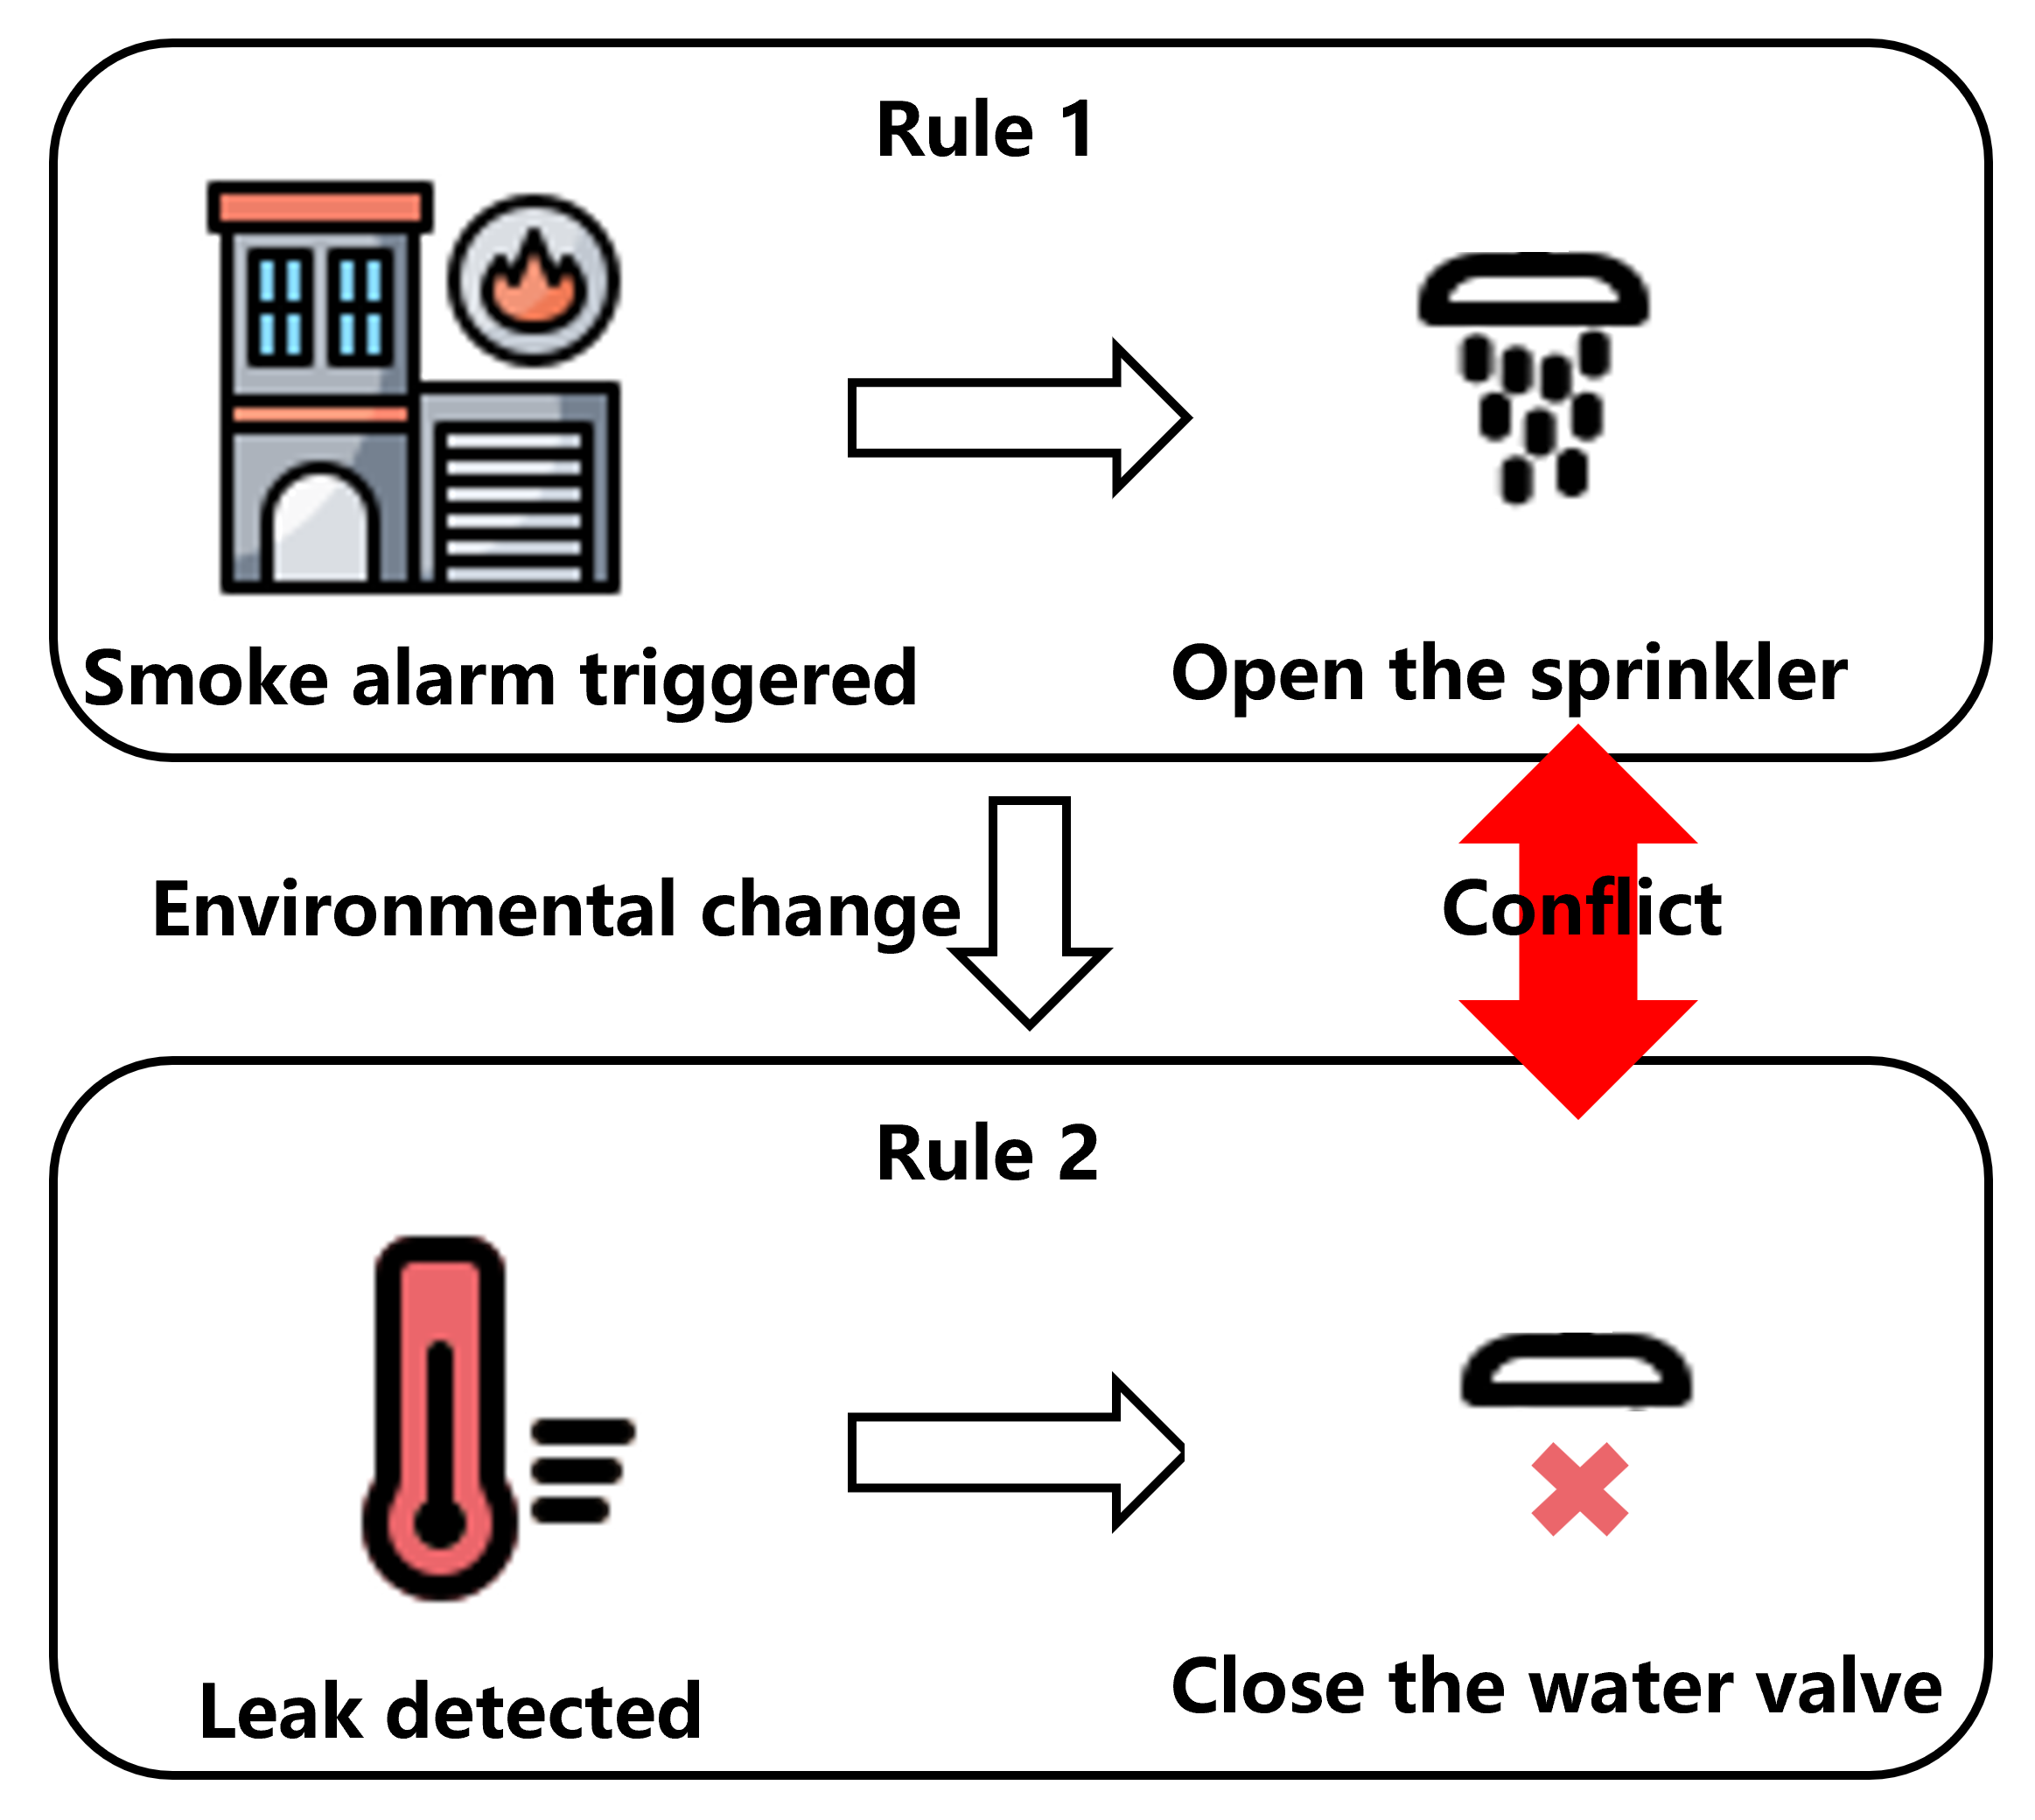
\includegraphics[width=0.4\textwidth]{figure/rule_conflict_example.png}
	\caption{Rule Conflict Example}
	\label{rule_conflict_example}
\end{figure}

%针对智能家居中存在的规则冲突问题,当前已经有了相关研究。规则冲突检测方法主要分为两类:(1)定义一些安全策略,如果检测到当前自动化规则的执行违反了安全策略,则判定为规则冲突;(2)根据自动化规则交互模式进行判断,如果满足规则交互模式则表示命中,即存在规则交互威胁。规则冲突检测的技术主要包括三类:(1)代发分析:对规则文件及逆行分析,查找可能存在的规则冲突;(2)模型检测,在自动化规则运行时通过模型检测等方法进行检测;(3)图分析,为应用程序生成控制流图,根据检测控制流的触发、条件、操作和逻辑条件推导实际系统中是否发生规则冲突。规则冲突的处理方法主要分为以下三类:(1)重新配置自动化规则;(2)设置特定的安全策略,当规则冲突发生时,保证执行结果不违反安全策略;(3)根据规则冲突定制处理方法,其本质上是另一种预定义安全策略,但是针对不同的规则冲突提供了多中的处理策略以供选择。
There has been relevant research on the problem of rule conflicts in smart homes. 
Rule conflict detection methods are mainly divided into two categories: 
(1) defining some security policies, and if it is detected that the execution of the current automation rule violates the security policy, it is determined as a rule conflict; 
(2) judging according to the automation rule interaction mode, and if the rule interaction mode is satisfied, it means a hit, that is, there is a rule interaction threat. 

The technologies for rule conflict detection mainly include three categories: 
(1) proxy analysis: analyzing rule files and reverse analysis to find possible rule conflicts; 
(2) model checking: detecting through model checking and other methods during the operation of automation rules; 
(3) graph analysis: generating a control flow graph for the application, and inferring whether a rule conflict occurs in the actual system according to the triggering, conditions, operations, and logical conditions of the detection control flow. 

Rule conflict handling methods are mainly divided into the following three categories: 
(1) reconfiguring automation rules; 
(2) Set specific security policies, which ensures that the execution result does not violate the security policy when a rule conflict occurs; 
(3) customizing the handling method according to the rule conflict, which is essentially another predefined security policy, but provides multiple handling strategies for different rule conflicts to choose from.

%当前的规则冲突解决方案在一定程度上缓解了规则冲突,但是仍存在一定的缺陷。
The current rule conflict resolution scheme alleviates rule conflicts to some extent, but still has some defects.

%在规则冲突检测方面:
In terms of rule conflict detection:
%\begin{itemize}
%	\item 检测智能家居系统是否违反安全策略来判断是否出现规则冲突,但是智能家居系统具有多样性,对于具体的系统不能照搬其他系统的安全策略,安全策略不完备表明该方法不能检测到所有可能存在的规则冲突。例如某个家庭设置了“检测到烟雾时喷头阀门开启”,但另一个家庭的规则中设定“明火检测警报后喷头阀门开启”,前一个家庭的规则可能不适用于第二个家庭。
%	\item 检测智能家居系统是否存在规则交互威胁,即是否满足某种规则交互模式,但是对于规则交互与规则冲突的界限模糊,容易产生假阳。例如存在两条规则,分别是“落日,开启暖气”和“温度达到30℃,打开窗户并关闭暖气”,这对规则在室内花园中可能有益,但是同样的规则内容作用于一楼的住户的卧室来说将会带来严重安全隐患。
%\end{itemize}

\begin{itemize}
	\item Detecting whether smart home systems violate security policies to determine rule conflicts, but smart home systems are diverse, and security policies of other systems cannot be directly applied to specific systems. Incomplete security policies indicate that this method cannot detect all possible rule conflicts. For example, one family sets "sprinkler valve opens when smoke is detected," but another family's rule sets "sprinkler valve opens after open flame detection alarm." The former family's rule may not apply to the latter family.
	
	\item Detecting whether there are rule interaction threats in smart home systems, i.e., whether a certain rule interaction pattern is satisfied. However, the boundary between rule interaction and rule conflict is blurred, which can easily lead to false positives. For example, there are two rules: "sunset, turn on the heating" and "when the temperature reaches 30 degrees Celsius, open the window and turn off the heating." These rules may be beneficial in an indoor garden, but the same rules applied to the bedroom of a first-floor resident will bring serious security risks.
\end{itemize}

%在规则冲突处理方面:
In terms of rule conflict resolution:
\begin{itemize}
	\item Modifying rule configuration may cause the rules to malfunction; modifying existing automation rules does not guarantee that no new conflicts will be introduced, and it cannot truly solve the problem.
	
	\item Using a general security strategy protects home safety to some extent, but the same security strategy does not apply to every household.
\end{itemize}

\begin{figure}[htbp]
	\centering
	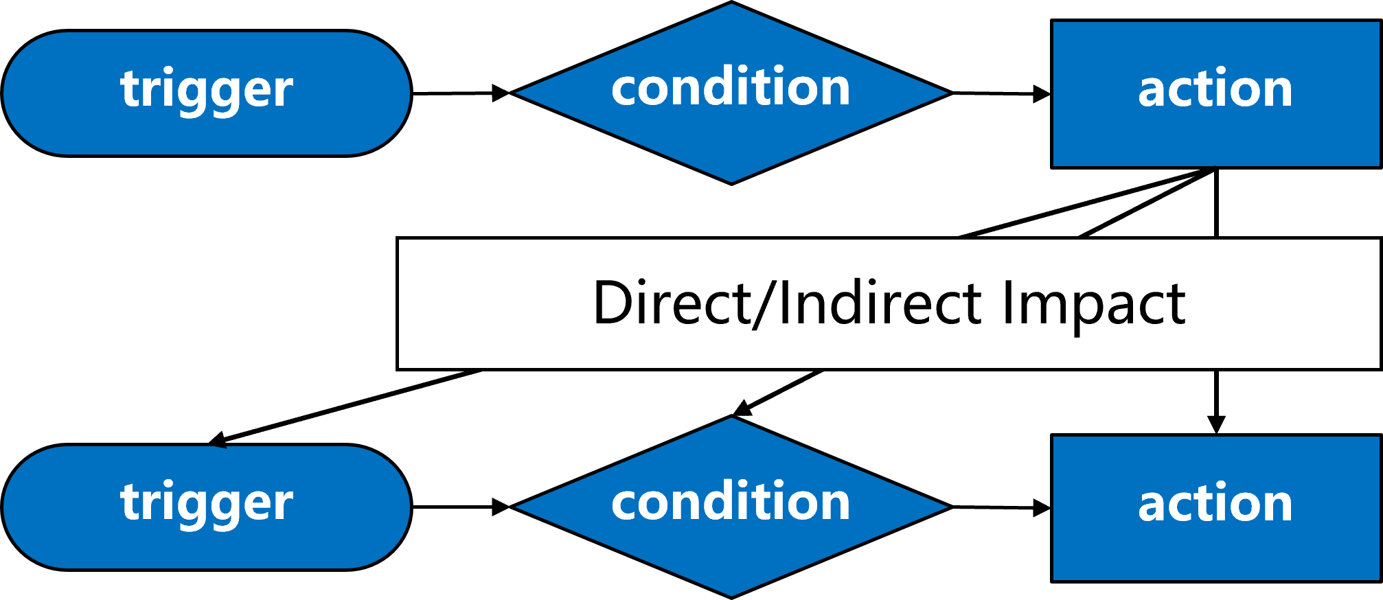
\includegraphics[width=0.4\textwidth]{figure/classification_observation.png}
	\caption{Rule Interaction Pattern}
	\label{classification_observation}
\end{figure}

%对于智能家居系统中的自动化规则交互,本论文的工作主要基于以下观察:(1)如Fig.\ref{classification_observation}展示,自动化规则之间的交互可以根据以下方法归纳为六种类型:一条规则执行的结果对另一条规则的触发器、条件与执行产生直接或者间接影响;(2)一个规则交互是否属于规则冲突的定义比较主观,根据用户个人偏好而定;(3)智能家居系统采用TCA模式实现自动化规则的触发判断与执行,可以考虑使用在系统间使用代码插装技术读取当前与历史执行的规则信息,从而进行规则冲突判断信息的获取与规则冲突处理。
For the automation rule interaction in smart home systems, the work of this paper is mainly based on the following observations: (1) As shown in Fig.\ref{classification_observation}, the interaction between automation rules can be summarized into six types according to the following methods: the execution result of one rule has a direct or indirect impact on the trigger, condition, and execution of another rule; (2) Whether a rule interaction belongs to a rule conflict is subjective and depends on personal user preferences; (3) The smart home system uses the TCA model to implement the trigger judgment and execution of automation rules, and it is possible to consider using code instrumentation technology between systems to read the current and historical executed rule information, so as to obtain rule conflict judgment information and rule conflict processing.

%本论文根据对规则交互模式的分析进行规则交互/冲突类型划分,为了考虑到间接影响引起的规则交互/冲突,结合用户的环境配置对规则重新建模,然后使用形式化分析进行模型检测,检测出可能存在的所有规则交互。结合用户对实体安全配置实现可以实现基本的规则冲突判断与冲突处理策略推荐,用户也可以结合个人偏好进行调整。智能家居系统基于TCA模型执行自动化规则,当规则冲突发生时,可以选择对两条规则的选择性执行,从而得到对于每对冲突规则的定制化处理策略,而非固定的通用安全策略。代码插装技术可以帮助获取系统中所有设备状态与历史自动化规则的执行信息,从而实现对系统的实时检测与冲突处理。
This paper classifies rule interaction/conflict types based on the analysis of rule interaction patterns. To account for rule interactions/conflicts caused by indirect influences, it remodels rules by incorporating user environment configurations. Then, it uses formal analysis for model checking to detect all possible rule interactions. By combining user security configurations for entities, it enables basic rule conflict detection and recommends conflict resolution strategies, which users can also adjust according to their preferences. The smart home system executes automation rules based on the TCA model. When rule conflicts occur, it can selectively execute the two rules, thereby obtaining customized handling strategies for each pair of conflicting rules, rather than fixed, general security policies. Code instrumentation techniques can help acquire the system's device states and historical automation rule execution information, enabling real-time system detection and conflict resolution.

%总结来说,本论文主要有以下贡献:
In summary, this paper makes the following contributions:

%\begin{itemize}
%	\item 规则运行机制的分析和规则冲突的分类:根据自动化规则运行机制对规则冲突进行分类,能够覆盖所有规则交互类型
%	\item 设计与实现结合静态和动态冲突检测的方案,实现一种适用于智能家居规则的广泛适用的冲突检测机制:对规则增加区域属性然后重新建模,结合安全实体配置进行自动化规则冲突静态检测,采用断言检测的方法在实时运行中检测系统中是否出现规则冲突
%	\item 设计与实现冲突解决方案、定制化的冲突规则处理策略,以及冲突预防措施的实现:根据自动化规则运行机制实现多种冲突处理策略,可以根据安全实体配置对规则冲突进行自动选择适合的处理策略,并在规则冲突发生前拦截防止发生规则冲突
%\end{itemize}
\begin{itemize}
	\item Analysis of the rule execution mechanism and classification of rule conflicts: Classify rule conflicts according to the automated rule execution mechanism to cover all rule interaction types.
	\item Design and implementation of a solution combining static and dynamic conflict detection to achieve a widely applicable conflict detection mechanism suitable for smart home rules: Add region attributes to the rules and remodel them, combine with security entity configuration for static detection of automated rule conflicts, and use assertion detection methods to detect whether rule conflicts occur in the system in real-time operation.
	\item Design and implementation of conflict resolution solutions, customized conflict rule handling strategies, and implementation of conflict prevention measures: Implement various conflict handling strategies according to the automated rule execution mechanism, automatically select appropriate handling strategies for rule conflicts based on security entity configuration, and intercept rule conflicts before they occur to prevent them from happening.
\end{itemize}
